\chapter{Hash Tables}
\label{ch:hash-tables}

In previous chapters, we have seen how lists can be used to store
multiple values, such as all the students in a class or all the books
in a library. Operators provide convenient access to the first element
in a list and to the elements after it, in sequence one by one.
%so all the elements of a
%list can be processed with operators that can be defined by inductive
%equations.
This is fine when you want to
process all the elements in the list, but what if you're only interested
in the student with ID \#93574 or Mary Shelley's ``Frankenstein; or,
The Modern Prometheus''?
Computer scientists have designed many
ways to get fast and convenient access
to individual records out of large collections.
In this chapter we'll study a solution known as \index{hash}\emph{hashing}.

\section{Lists and Arrays}

Suppose we have a list of states and their
\label{states-capitals-list}capitals.
\begin{center}
\begin{tabular}{lll}
\textsf{[} &\textsf{["Alabama"}  &\textsf{"Montgomery"]}\\
  &\textsf{["Alaska"}   &\textsf{"Juneau"]}\\
  &\textsf{["Arizona"}  &\textsf{"Phoenix"]}\\
  &~~~$\vdots$     &\\
  &\textsf{["Wyoming"}  &\textsf{"Cheyenne"] ]}\\
\end{tabular}
\end{center}

\begin{figure}
\begin{center}
Axioms for Finding State Capitals
\begin{spacing}{0.9}
\begin{tabular}{lll}
\hline
(capital $s$ nil) = nil                               &             & \{\emph{cap0}\} \\
(capital $s$ (cons [$state$ $city$] $caps$)) = $city$ &if $s=state$ & \{\emph{cap1}\} \\
(capital $s$ (cons [$state$ $city$] $caps$)) = (capital $s$ $caps$) & if $s \neq state$ & \{\emph{cap2}\} \\
\end{tabular}
\end{spacing}
\begin{code}
\begin{verbatim}
(defun capital (s caps)
 (if (consp caps)
     (if (equal (first (car caps)) s)
         (car (rest (first caps)))
         (capital s (rest caps)))
     nil))
\end{verbatim}
\end{code}
\caption{Operator to Find State Capitals}
\label{fig:state-capital-operator}\index{operator, by name!capital}\index{search!array}\index{array!search}
\end{center}
\end{figure}

Figure~\ref{fig:state-capital-operator}
defines an operator to find the
capital of any given state, given such a list.
The operator works, but it's slow.
It takes only a handful of steps to find the capital of Alabama,
but it takes fifty steps to find the capital of Wyoming.
Some states are near the front of the list,
others far down the list.
If a queries are as likely to ask about
one state as another,
then on the average it will take twenty-five steps to find
the state capital requested by a query.
The situation would be worse for a bigger problem,
such as finding the population of a city in a list of city/population pairs.
In other words, the solution works but doesn't scale well.

Chapter~\ref{ch:search-trees} discusses the binary search
method (page \pageref{binary-search-method}),
which is a way to speed up the process of finding an item
(such as a capital city)
associated with a search key (such as a state name) in a
collection of items. The chapter goes on to discuss
a data structure known as a binary tree
that provides an effective solution to the search
problem.\footnote{Chapter~\ref{ch:search-trees}
discusses a particular kind of binary tree known as an AVL tree,
but that is just one of many kinds of trees
that can be used to solve the problem of searching
for data associated with keys.}
Binary trees would make it possible to find
state capitals faster
than the operator of Figure~\ref{fig:state-capital-operator}.
The states and capitals would need to be stored
in a special way, not an ordinary list,
but the number of steps required to find a capital
would drop from an average of twenty-five to a maximum of six.
That's four times faster, but there is a method known as hashing %'
that cuts the search to something close to one step, or at least
to a small number of steps, regardless of how
many search keys are in the data.
Hashing works well for data sets that don't change often, %'
such as state capitals. It works less well for large
data sets that change frequently, such as tweets.
You have to choose a solution that fits the problem.
Hashing provides one alternative.

Part of the problem with using ACL2 lists
for data is that it is easy and fast to retrieve the
first element of a list, but slower to retrieve the
$n$\textsuperscript{th} element of a list.
However, that's not the whole problem. %'
It also takes time to compare search keys
(state names, in the problem at hand).
Hashing addresses that problem by converting the search key
into a numeric index and putting the data
in an array providing one-step access by index.

There is an ACL2 operator called \textsf{nth} that,
given an index and a list, delivers the
$n$\textsuperscript{th} element of the list.
Indexes start at zero, so the index
zero selects the first element,
the index one selects the second element,
and so on.\footnote{Most people
count things starting from the number one (1, 2, 3, \dots), but
computer scientists usually start from zero (0, 1, 2, 3, \dots)
for reasons that have to do with the simplicity
of formulas for indexes in some contexts, such
as when an index selects a polynomial coefficient
or when elements are grouped in blocks.
It seems odd to count from
zero instead of from one,
but that's the way the operator
\textsf{nth} does its indexing. We're stuck with it.}
If we let \textsf{states} stand for the list of states and capitals
(page \pageref{states-capitals-list}), then
\textsf{(nth 1 states)} is \textsf{["Alaska" "Juneau"]},
while \textsf{(nth 0 states)} is \textsf{["Alabama" "Montgomery"]}.

\begin{center}
Axioms for \textsf{nth} operator
\begin{tabular}{ll}
\textsf{(nth 0} $xs$\textsf{)} $=$ \textsf{(first} $xs$\textsf{)}  & \{\emph{nth0}\}             \\
\textsf{(nth} $n+1$ $xs$\textsf{)} $=$ \textsf{(nth} $n$ \textsf{(rest} $xs$\textsf{))} & \{\emph{nth1}\} \\
\end{tabular}
\end{center}

However, the \textsf{nth} operator is a slow way to reach a
list-element that has a high index.
An array is a data structure that is
similar to a list, but it provides fast access to its
elements, including those with a high index.
If the list of states and capitals were recorded in an array instead
of a list, it would be just as fast to find the entry for the
fiftieth state (Wyoming) as it is to find the entry
for the first state (Alabama).

Suppose the operator \textsf{nth} could be implemented
in such a way that it would not take any longer to
deliver the element with index $1,000,000$ than it would take
to deliver the element with index $0$.
Let's not worry about how that could be done, but %'
just assume for the moment that ACL2 could do it.
If \textsf{nth} were such an operator,
how much faster would the operator \textsf{capital} be?

A fast implementation of \textsf{nth} is part of the answer,
but not a complete solution to finding state capitals
with a one-step operation.
We still need to find the right state.
That is, it still takes many steps to find Wyoming.
Hashing solves the problem of finding any search key fast.

\begin{aside}{aside:arrays-and-acl2}{Arrays and ACL2}
Lists are one way to maintain collections of data in ACL2,
but not the only way. A data structure
known as an array is another. It comes with an operator
called \textsf{aref1} that retrieves values from array elements.
It is similar to the hypothetical, ``fast \textsf{nth}'' operator
discussed in this section. However, using ACL2 arrays in a way that
ensures that \textsf{aref1} retrieves elements fast
is a complicated, technical procedure.
Acquiring the required ACL2 expertise to use arrays
would take us too far afield, so we will rely on a
descriptive approach that omits the details.
%\caption{Arrays and ACL2}
\end{aside}

\section{Hash Operators}

We are looking for a definition of the operator
\textsf{capital} that, given a state, finds right entry
in the list of state/capital pairs.
We will assume that the formula \textsf{(nth} $n$ $xs$\textsf{)}
completes its retrieval of element $n$ from the list $xs$
in one step. That is, we are assuming that a hypothetical,
fast version of \textsf{nth} exists. It doesn't, but the
array facilities in ACL2 make an operator like that possible,
so when we write a formula like
\textsf{(nth} $n$ $xs$\textsf{)},
we think of $xs$ as an array and assume that
\textsf{nth} is a one-step operation.

Our first solution to the search problem is alphabetical.
It's not a complete solution, but will help us move in that direction.
We will use array of 26 elements
and put all states that start with the letter A in
the element with index zero,
the ones with that start with B in the element with index one, and so on.
Since there are 50 states and only
26 elements in the array, some elements will have more than one state,
so searching as before will still be necessary, but shorter.
Finding Kansas, for example, will be
a matter of retrieving the array element associated with
the letter K, then sorting through the states in that entry.
There are two states that start with K,
so it will take at most two more steps after retrieving
the array element for K.  Let's assume that's about
average.\footnote{If the first letters in state names
were evenly distributed across the alphabet, there would be
two entries in most elements of the array, so the number of steps
for Kansas would be more-or-less typical.
Of course, some letters are associated with more states than
others, so it's not always going to be a matter of finding
the letter and picking between two states. There are eight
states that start with M, so it can get bad,
but the average for array elements with states in them
is about 2.6 states per array element, so
\index{Kansas}Kansas isn't far from average.}
That is, after retrieving the array element corresponding to
the first letter in the name of the state, there will
be typically about two states in the box.

\begin{figure}
\begin{center}
Letterbox Array: \textsf{fcaps}
\begin{tabular}{c|l}
\emph{Index} &\emph{State Capitals} \\
\hline
0 & \textsf{[ ["Alabama"  "Montgomery"] ["Alaska"   "Juneau"] \dots } \\
  & \textsf{~~\dots ["Arkansas"  "Little Rock"] ]}  \\ %[arizona  phoenix]
1 & \textsf{[ ]}\\
2 & \textsf{[ ["California"  "Sacramento"] ["Colorado"  "Denver"] \dots } \\
  & \textsf{~~\dots ["Connecticut"  "Hartford"] }]\\
3 & \textsf{[ ["Delaware"  "Dover"] ]}\\
%\multicolumn{2}{c}{\vdots} \\
\vdots & \hspace*{15mm}\vdots\\
\end{tabular}
\begin{tabular}{lll}
\multicolumn{3}{c}{Axioms for Capital Search Operator: \textsf{fcapital}}\\
\hline
\textsf{(fcapital} $s$ \textsf{fcaps)} $=$ \textsf{(lookup} $s$ \textsf{(nth (state-idx} $s$) \textsf{fcaps))} && \{\emph{fcap}\} \\
\textsf{(lookup} $s$ \textsf{nil)} $=$ \textsf{nil}  && \{\emph{look0}\}     \\
\textsf{(lookup} $s$ \textsf{(cons (cons} $state$ $city$\textsf{)} $caps$\textsf{))} $=$ $city$ &if $s = state$ & \{\emph{look1}\} \\
\textsf{(lookup} $s$ \textsf{(cons (cons} $state$ $city$) $caps$\textsf{))} $=$ \textsf{(lookup} $s$ $caps$\textsf{)} &if $s \ne state$ & \{\emph{look2}\} \\
\end{tabular}
\end{center}
\index{letterbox array}\index{state capitals}\index{capitals of states}\index{operator, by name!fcapital}\index{operator, by name!lookup}\index{operator, by name!state-idx}\index{search!array}\index{array!search}
\caption{Letterbox Array and Capital Search Operator}
\label{fig:fcaps-array}
\end{figure}

Let's call this an array of letterboxes
(one array element for each letter in the alphabet)
and give it the name \textsf{fcaps}.
It represents the same information as the earlier list, \textsf{states},
but in a form that makes finding a state capital faster.
We call the new operator for finding the capital of a state
\textsf{fcapital} (``f'' for fast).
It delivers the same results
as the previous operator, \textsf{capital},
but does so in fewer steps because the information in its array operand,
\textsf{fcaps}, is arranged to shortens the search.
Figure~\ref{fig:fcaps-array} suggests the contents of a few
of the letterboxes in \textsf{fcaps} and presents some
equations defining \textsf{fcapital}.

The \textsf{fcapital} equations refer to an operator
called \textsf{lookup} that, like the operator, \textsf{capital},
returns the matching element from a list of state/capital pairs.
We could have stuck with the previous operator,
but \textsf{lookup} searches short lists,
typically one to three elements,
whereas \textsf{capital} had to deal with all fifty states.
In a working system,
a better definition of \textsf{lookup}
would take advantage of the special nature of the data set.

We want to focus on the definition of \textsf{fcapital},
which does most of the work.
The operator \textsf{fcapital} invokes \textsf{lookup}
on the letterbox corresponding to the first letter
in the name of the state.
The operator \textsf{state-idx} computes the index
of the letterbox, given the name of a state:
0 for Alabama or Arkansas, 2 for California,
3 for Delaware, \dots 22 for  Wyoming.
We will leave the concrete
definition of \textsf{state-idx} as an exercise for
people who want to delve into the arcane details of
operations like retrieving the first letter from a
\index{string}string.\footnote{We use the term \emph{string}
to mean a sequence of characters.
Most programming languages, including ACL2,
denote strings by putting double-quote marks
around the characters: \textsf{"This is a string."}}
Those details are necessary to build a working system,
but they don't add much to the discussion of ways
to retrieve data quickly from a data set.

The formula
\textsf{(nth (state-idx $s$) fcaps)}
retrieves a letterbox from the array \textsf{fcaps}.
The version of \textsf{nth} that we refer to here
is the hypothetical operator that we discussed earlier,
which in a single step delivers an element
with the specified index from an array.
We didn't say how that operator worked.
It can be done. We leave it at that.

We want to figure out
how well the idea of having one box for each letter
in the alphabet works.
There 50 states and 26 letters, but the letters occur
with different frequencies in state names.
There are four states that start with A and
eight that start with M,
but none that start with B or E.
It would be better to put the same number of states in each
array element. We could, for example have 25 boxes and put
two states in each box. Or, we could have 50 boxes, and put
one state in each box.
We could even have a hundred boxes and put one state in 50
of the boxes and no states in the other 50.
Sounds stupid, but it's not, depending on how
the \textsf{state-idx} operator is defined,
and we will talk about that shortly.

In any case the \textsf{lookup} operation could be faster
if the states were distributed more evenly among the boxes.
To make that work, the definition
\textsf{state-idx} would need to be more sophisticated
the just going by the first letter in the name of the state.
It would need to use more letters in the name
to compute the index of the box containing the corresponding
state/capital pair.

Choosing a way to distribute the states among the boxes
and defining a special version of \textsf{state-idx}
to compute the index of the right box is
more art than science. This kind of problem comes up in
many kinds of table-lookup problems. We are using
state capitals as an example to discuss the issues,
but the problem of looking up information associated
with URLs is the same, only bigger and more complicated.
For example the first ten characters in the URL
http://www.apple.com/ are the same as the first ten
characters in http://www.cnn.com/. The last five
characters are the same in both URLs, too.
So, if we distribute all the URLs into an array of URL-boxes,
defining an operator, say \textsf{URL-idx}, to compute the
index of the box containing a given URL,
then the operator \textsf{URL-idx} should take
all of the characters in the URL into consideration.
We have the same problem with state names, but on a
smaller scale, so let's get back to that discussion.

There are many ways to set up the letterboxes.
They are not ``letterboxes'' anymore, but boxes set up to hold
state/capital pairs distributed into those boxes using
more than just the first letter in the name of the state.
We will refer to them as the
\index{bucket, hash}\index{hash!bucket}\emph{buckets}
of the \index{hash!table}\emph{hash table}.
(Yes, we're going to call them buckets. It's hashing terminology.)
And, the definition of \textsf{state-idx} must be
tailored to the way the states are distributed among the buckets.
Some distributions of states and corresponding definitions
of \textsf{state-idx} work better than others.
The key is to look at more letters in the name of the state
than just the first one.
Choosing the details of the distribution of keys
(state names in our example) and the definition of the index operator
(\textsf{state-idx} in our example) is where the art comes in.
The trick is to choose a distribution and operator
definition that makes for a fast \textsf{state-idx} operation.

Let's discuss this problem in a more general context
where the keys are strings of characters that we will
call \emph{words}, even though they might be odd-looking
strings like URLs.
A common solution is to use two steps. First, the word,
which we refer to as the search key, is converted
into a list of numbers by mapping each character to a number. For
example, we could convert A to 1, B to 2, C to 3,
and so on.\footnote{This is not the usual scheme,
and we're conflating upper- and
lower-case letters, but other number/letter conversions  will also work.}
Using the A 1, B 2, C 3 scheme, the word ``life'' becomes the list
\textsf{[12 9 6 5]},
and the word ``file'' becomes \textsf{[6 9 12 5]}.

The second step is to take the list of numbers corresponding
to the letters in the search key
and combine them into a single number called
the \index{hash!key}\index{search!hash}\index{hash!search}\emph{hash key}.
The operator that computes the hash key is called
the \index{hash!operator}\emph{hash operator}.
Ideally, the hash operator associates a different hash key
with each search key.
One way to compute a hash key from the list of numbers
corresponding to the letters in the search key is
to add multiples of powers of a
prime number, which is called the
\index{hash!base}\emph{hash base}.\footnote{Why choose a prime?
There is a lot of number theory involved in these kinds
of problems, but that's a story for a different book.
We'll leave it as a mystery.}

If we choose the prime number $31$
as the hash base, the list \textsf{[12 9 6 5]} maps to the hash key
$12 + 9\times31 + 6\times31^2 + 5\times31^3 = 155,012$.
The numbers 12, 9, 6, and 5 are used as coefficients to powers of
the hash base.\footnote{This treats the
list of numbers as a base-31 numeral, as
discussed in Chapter~\ref{ch:binary-numerals}.
It may happen that some of the digits in the numeral
fall outside the usual range for base 31 digits,
but the method in Chapter~\ref{ch:binary-numerals}
for computing numbers from numerals works
for the hash-key computation, too. Not in the other direction, though.
The hash coefficients can't be computed from the hash key.}
The list \textsf{[6 9 12 5]} maps to the hash key
$6 + 9\times31 + 12\times31^2 + 5\times31^3 = 160,772$.
That might be okay if there were hundreds of thousands of words
that need to be associated with indexes, as there would be
if the words were URLs, for example.

In the problem at hand, there are fifty states,
so there are fifty search keys.
Let's get back to that again.
The \textsf{fcapital} operator uses the
number returned from \textsf{state-idx} as an index to
an element in the array containing the (short) lists of
state/capital pairs, in which
\textsf{lookup} will find the capital of the state.
A hash table with 160,772 elements is overkill for
a problem with fifty search keys.
We had a hash table with 26 elements when we used the first letter of the state.
Suppose we look for a solution with a hash table of a hundred elements.
Then, we would need to compute hash index between zero and ninety-nine
from the hash key. One way to do that would be to
consider only the last two digits of the hash key.
Then, the hash index for the hash key 160,772 would be 72.
The word ``life'' (not the name of a state, but you get the idea)
would go into the bucket
with index 72.
There's nothing special about 100.
If we wanted a fifty-bucket solution,
we could compute the index from the hash key by taking the
remainder in the division\footnote{Box~\ref{third-grade-division},
page \pageref{third-grade-division} discusses
division, remainders, and the $mod$ operator.}
by  $50$: ($160,772$ $mod$ $50$) = $22$.
The method works for a hash table with any number of buckets.

To pick a hash base and hash table size
that works well is a matter of analyzing how
the hash keys come out for the words we want to look up.
If we want to extend this problem to take into
account Canadian provinces or all the countries in the world, we could
use an array with, say, a thousand elements.
The hash operator could compute a hash key $h$ from a search key,
as before, then deliver ($h$ $mod$ $1,000$) as the hash index.

We've discussed a lot of ideas in this chapter
that are important and practical in computer science.
Let's take a moment to recap these ideas.
The general problem we set out to solve was how to find quickly a value
associated with a name. In general, we think of having many key/value pairs,
and what we'd like to do is to find the \emph{value} associated with a given
\emph{key}. This general problem is so important that many computer languages
offer ready-made solutions, which are called by
various names: \emph{associative arrays}, \emph{dictionaries},
\emph{maps}, \emph{memories}, and others.
We call them hash tables in this discussion,
but they are all similar ideas.

The first solution we discussed was
to keep all the key/value pairs in a single list
and search for keys by going through the list, one by one.
This works, but is too slow to scale up.
On the average, if search keys all have about the same likelihood of
being the target of a search,
the search will have to look at roughly half
of the key/value pairs before it finds the one it's looking for. %'
For many, real-world problems, that is too long.
A hash table alleviates this problem
by splitting the list of key/value pairs into many smaller lists.
Each of these lists goes into one of the buckets of the hash table.
With this approach the time required to locate a key
will be, at worst, proportional
to the number of search keys in the biggest bucket,
which is much smaller than the total number of search keys.
There is a trade-off between the number of buckets and the size of the buckets.
Smaller buckets, faster search, but more total space because,
depending on how the hash index is computed,
there can be a lot of empty buckets
that take up space even though they are empty.

The big question is how to distribute the key/value pairs into the various buckets.
That is determined by the hash operator and
the computation of the hash index from the hash key.
The goal in designing hash operators and hash tables
is to put about the same number of search keys in each bucket.
A popular hash operator for
strings is to treat each character as a number, to use these numbers as the
coefficients for a sum of powers of 31, and then to trim that number to
a hash index by computing the remainder in the division by
the number of buckets in the hash table.
This overall process is illustrated in Figure \ref{fig:hash-table-process}.

\begin{table}
\begin{center}
\begin{tabular}{c|p{4in}}
\emph{Bucket} & \textsf{[}\emph{key value}\textsf{]} \emph{Pairs} \\
\hline
0 & \textsf{["Washington" "Olympia"]  ["Utah"  "Salt Lake City"]}  \hfill\break
\textsf{["Rhode Island"  "Providence"]  ["New Hampshire"  "Concord"]}  \hfill\break
\textsf{["Minnesota"  "St Paul"]  ["Kentucky"  "Frankfort"]} \\
\hline
1 & \textsf{["Nebraska"  "Lincoln"] ["Louisiana"  "Baton Rouge"]} \hfill\break
\textsf{["Hawaii"  "Honolulu"]  ["Alabama"  "Montgomery"]} \\
\hline
2 & \textsf{["Pennsylvania"  "Harrisburg"]  ["New York" "Albany"]} \hfill\break
\textsf{["New Mexico"  "Santa Fe"]  ["Maine"  "Augusta"]} \hfill\break
\textsf{["Indiana"  "Indianapolis"]  ["Georgia"  "Atlanta"]} \\
\hline
3 & \textsf{["Missouri"  "Jefferson City"]  ["Colorado"  "Denver"]} \\
\hline
4 & \textsf{["Oregon"  "Salem"]  ["Michigan"  "Lansing"]} \hfill\break
\textsf{["Arkansas"  "Little Rock"]  ["Arizona"  "Phoenix"]} \\
\hline
5 & \textsf{["Wisconsin" "Madison"]  ["New Jersey"  "Trenton"]} \hfill\break
\textsf{["Kansas"  "Topeka"]  ["Florida"  "Tallahassee"]} \hfill\break
\textsf{["Alaska"  "Juneau"]} \\
\hline
6 & \textsf{["Wyoming"  "Cheyenne"]  ["Tennessee"  "Nashville"]} \hfill\break
\textsf{["South Dakota"  "Pierre"]  ["Oklahoma"  "Oklahoma City"]} \\
\hline
7 & \textsf{["West Virginia"  "Charleston"]  ["Vermont"  "Montpelier"]} \hfill\break
\textsf{["South Carolina"  "Columbia"]  ["Ohio"  "Columbus"]} \hfill\break
\textsf{["Nevada"  "Carson City"]  ["Mississippi"  "Jackson"]} \hfill\break
\textsf{["Idaho  Boise"]  ["Connecticut"  "Hartford"]} \\
\hline
8 & \textsf{["North Dakota"  "Bismarck"]  ["Montana"  "Helena"]} \hfill\break
\textsf{["Massachusetts"  "Boston"]  ["Maryland"  "Annapolis"]} \hfill\break
\textsf{["Iowa" "Des Moines"]  ["California"  "Sacramento"]} \\
\hline
9 & \textsf{["Virginia"  "Richmond"]  ["Texas" "Austin"]} \hfill\break
\textsf{["North Carolina" "Raleigh"]  ["Illinois"  "Springfield"]} \hfill\break
\textsf{["Delaware"  "Dover"]} \\
\end{tabular}
\end{center}
\caption{Ten-Bucket Hash Table for State Capitals}
\label{table:hash-table-state-capitals}
\end{table}

In our state/capital example the search keys were state names and the
associated values were capital cities.
Using a hash table with ten buckets and the hash operator
we discussed, the key/value pairs would be associated with the
buckets as seen in
Table \ref{table:hash-table-state-capitals}
(page \pageref{table:hash-table-state-capitals}).
As the table shows, the states are not distributed evenly in the
buckets. Bucket 7 has
eight states, but bucket 4 has only two.
Keeping the same hash operator but using thirty buckets
instead of ten does a better job of distributing states to buckets.
Keeping the hash operator separate from the number of buckets
makes it easy to change the size of the
hash table, depending on how fast the search needs
to be.\footnote{For small problems like the state/capital problem,
there are mechanized ways to design hash operators and
hash arrays that lead to \index{perfect hash}\index{hash!perfect}\emph{perfect hashes} with no
more than one key in each bucket. Sometimes there are
empty buckets, but that doesn't affect the search time,
just takes up more space. Some of the methods of
finding perfect hashes also provide ways to economize
on the number of buckets.
Hashing is an important and well studied search method.
You might find it interesting to look into the topic in more depth.}

\begin{figure}
\begin{center}
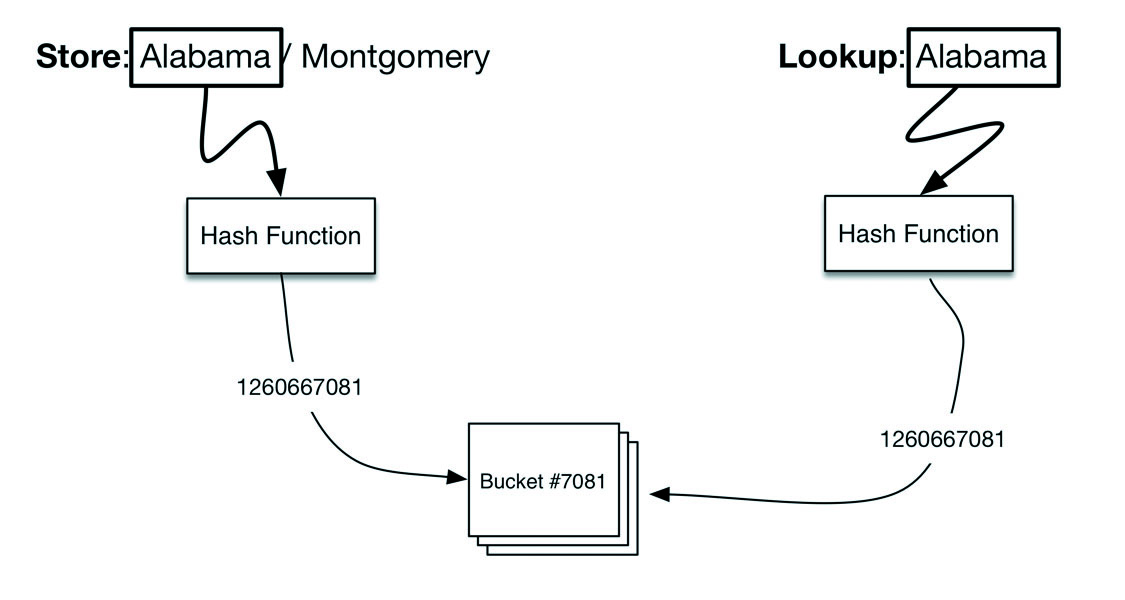
\includegraphics[scale=1]{images-cmyk/hash-table-process}
\end{center}
\caption{Hash Table Storage and Retrieval}
\label{fig:hash-table-process}
\end{figure}

\begin{figure}
\begin{center}
\begin{code}
\begin{verbatim}
(defun hash-op (hash-base chars)
   (if (consp chars)
       (+ (char-code (first chars))
          (* hash-base (hash-op hash-base (rest chars))))
       0))
(defun hash-key (hash-base wrd)
   (hash-op hash-base (coerce wrd 'list)))
(defun hash-idx (hash-base num-bkts wrd)
   (mod (hash-key hash-base wrd) num-bkts))
(defun rep (n x)
  (if (posp n)
      (cons x (rep (- n 1) x)) ; {rep1}
      nil))                    ; {rep0}
(defun bump-bkt (idx bkts)
   (if (posp idx)
       (cons (first bkts) (bump-bkt (- idx 1) (rest bkts)))
       (cons (+ 1 (first bkts)) (rest bkts))))
(defun fill-bkt-counts (hash-base num-bkts bkts wrds)
   (if (consp wrds)
       (let* ((idx (hash-idx hash-base num-bkts (first wrds)))
              (newbs (bump-bkt idx bkts)))
          (fill-bkt-counts hash-base num-bkts newbs (rest wrds)))
       bkts))
(defun hash-bucket-sizes (hash-base num-bkts wrds)
   (fill-bkt-counts hash-base num-bkts (rep num-bkts 0) wrds))
(defconst *example-tbl-25-most-common-English-words*
   (hash-bucket-sizes 31 10
      (list "the" "be" "to" "of" "and" "a" "in" "that" "have" "I"
            "it" "for" "not" "with" "he" "as" "you" "do" "at" "this"
            "but" "his" "by" "from" "they")))
\end{verbatim}
\end{code}
\caption{Prototype Hashing Operators (slow: using lists, not arrays)}
\label{fig:hash-defuns}
\end{center}
\end{figure}

\begin{exercises}
\exer {Consider the words ``age'', ``cage'', and ``cape''.
Using the hash operator from this chapter, compute the hash key of each word
and the bucket the word maps to, assuming there are ten buckets.}

% NOTE: I took this exercise out because it's a very big project
%       and it calls for a lot of knowledge of ACL2 that we haven't
%       even hinted about, such as what form to use for input.
%       I guess it would be feasible (albeit a lot of busywork)
%       to do it with symbols and single quotes, but I don't want to
%       go into those issues in any detail. Too much ACL2 programming.
%\Exercise Implement the operator \textsf{state-idx} in ACL2. For this
%project, you will need to read about the built-in operators \textsf{char},
%\textsf{char-code}, and \textsf{coerce}
%in the online ACL2 documentation.
%Don't worry about whether 'A' is 1,
%'B' is 2, and so on. Any number will do, so just use the one that
%\textsf{char-code} delivers.

\exer {There are many websites in the Internet that contain lists of words:
most popular baby names, most popular English words, etc.\\
\hspace*{5mm}\url{https://www.babycenter.com/top-baby-names-2017.htm} \\
\hspace*{5mm}\url{https://www.englishclub.com/vocabulary/common-words-100.htm}\\
Pick a list of words and explore how the hash operator of this chapter works.
Use 31 for the hash base and try different sizes for the hash table.
In your project, try to answer the following questions.}
\subexer {How many search keys are there in the biggest bucket?}
\subexer {What is the average number of search keys in a bucket?}
\subexer {How many empty buckets are there?}
\subexer {What is the average length of a non-empty bucket?}
\subexer {Which one of these measures best estimates how well this hash works?}
\begin{quote}
You can use the operators defined in
Figure~\ref{fig:hash-defuns} (page \pageref{fig:hash-defuns})
to get started on the project.
The operators use lists instead of arrays, so they are only  prototypes
for experimentation, not for practical use.
The definitions invoke some ACL2 intrinsic operators
that have not been discussed, such as
\textsf{coerce} and \textsf{char-code}.
The \textsf{coerce} operator converts a string to a list of characters,
and the char-code operator converts a character to a number.
The numbers are not the A 1, B 2, C 3, \dots, but that is immaterial.
Different characters are associated with different numbers,
which is the important thing. If you are interested,
you can find more information about these intrinsic
operators in the ACL2 online documentation.
\end{quote}
\end{exercises}

\section{Some Applications}

Hash tables provide an effective solution to the search problem,
so it is no surprise that they are all around us.
Hash tables are used behind the scenes in all sorts of applications.
They are ubiquitous computation.
Let's discuss some examples.

Hashing facilitates finding the definitions of operators
to run computer programs.
When you run a computer program,
the computer system needs to find the definitions
of the operators the program uses.
For example, the computer needs to know the definition of
\textsf{append} to compute the value of \textsf{(append [1 2] [3  4])}.
A lot of searches of this kind are required to run a program,
so a fast lookup procedure is important.

Hash tables offer a way to do it. Store the operator
definitions in a hash table where the key is the name of the operator
and the value is the definition. This is almost certainly the solution
that your computer system uses when it runs your ACL2 programs.
Another viable alternative is to use a binary search tree
(Chapter \ref{ch:search-trees}), but hash tables work better
in this situation because there are a moderate number of search keys
(operator names), and they don't change very often.
With a binary search approach and, say, a few hundred keys,
a binary search would have five or ten computational steps,
while a good hash operator and corresponding hash table
might find operator names several times faster.

The number of steps in binary search is proportional to the
logarithm of the number of keys. That's a lot less than a the
number of keys, but it does grow slowly as the number of keys increases.
The amount of time it takes to perform a search using a hash table
is proportional to the number of keys in the biggest bucket.
Of course, the computation of the hash key and bucket index
also has to be factored in, but whether the number of search keys
is a hundred or several thousand, the time takes to find a search
key stays about the same.

Database systems, the original killer app of
computing, are another common use of hashing.
Some of the earliest databases were used to keep track
of airline reservations, and now databases are used to store and
process all kinds of data: student records at a university,
transactions at every register in every Walmart,
cast members for every movie produced in Hollywood,
lifetime medical records for billions of people.
Organizations use databases to store literally
thousands of records related for each person involved in the system,
which can easily amount to billions
of records for an organization as a whole.

But, what is a database system? At its core, a database system
manages one or more tables, and each table is made up of one or more
records consisting of several attributes.
Think of a database table as a
spreadsheet, where each record corresponds to a row in the spreadsheet
and each column corresponds to an attribute. If the table
records states and their capitals, each database
record (or row in the spreadsheet) would have one attribute for the
state name and another attribute for the capital.

It is common to design a database table in such a way that the
data in a particular attribute is sufficient
to single out a specific record in the database.
For example, a table containing student records might use the attribute
``Student ID'' to identify each student, so there would be
a column in the table containing student IDs.
Given a student ID, the
database system can find the record for that student in the
table. Part of the magic of database systems is that they can retrieve
records quickly using specialized data
structures called \emph{database indexes}.
Database systems use indexes to retrieve specific records quickly,
even when the table has millions of records that are stored
in separate files on disk drives.

So, what is a database index? Database systems
offer many different kinds of indexes, but there are two kinds that are
the most common. One is based on hashing, the other on trees.
In a sense, a database
table is a key/value pair, where the key is an attribute that is
sufficient to identify a particular record and the value is the record
it identifies.

Hash-based and tree-based indexes
in databases are,
in essence, hash tables similar to those in this chapter
and trees similar to those of Chapter~\ref{ch:search-trees}.
The only substantial difference
is that our trees and hash tables are ACL2 objects that
to reside in the fast-access memory of a computer,
whereas database indexes are designed to retrieve records
that can be stored in very large files.

However, database systems go beyond storing and retrieving records
using a key. They also excel at finding information by combining
records in different tables. For instance, one table may have
information regarding a student's permanent address and another table
may have information listing the students enrolled in any given course.
A database query can combine these tables to find the zipcodes that
the students in any given course come from, perhaps showing that students in one
region of the country are more likely than those in another region to
enroll in history courses. That's the sort of insight that
data scientists find valuable.

Combining separate tables in a database can be expensive.
One way to proceed is to consider all possible pairs.
In the zipcode example, you could look at each course,
one at a time, and for each course consider
all the students who could be enrolled in it.
At a mid-sized university with 13,000 students
and 80,000 enrollment records, that would require
looking at over a billion combinations (1,040,000,000, actually).

Hash tables provide a simpler alternative. The student information table
and the course enrollment table are connected through the student ID.
So, before combining these tables, it is advantageous to hash both of them
using the student ID. Once this is done, each bucket contains some entries
from the student table and some from the course enrollment table. The entries
in each bucket must be considered exhaustively, but there is less work to do
than before.
To see this, suppose that there are 1,000 buckets,
each having an average of 13 students and 80 courses. Each bucket
contains $13 \times 80 =1,040$ combinations,
for a total of 1,040,000 combinations.
That makes retrieval a thousand times faster than the direct approach.

The reason that hash tables work so well in this context is that they take
a big problem and turn it into many smaller problems. Instead
of combining two tables of size 13,000 and 80,000, you can combine 1,000
tables of size 13 and 80. This savings is significant in itself, but it can
be even more dramatic if the smaller problems can be performed on different
computers. For example, if you have 1,000 computers, each one of them can be
working on a different bucket, so the total time to find the answer is
just the time to consider 1,040 combinations, which is a million times
faster than the direct approach.
This is kind of thing that companies with very large databases do---Google, Facebook, and Amazon, for example.
They use thousands of computers to process databases, and
hash tables are the key to spreading
the work evenly across the available computers.

Another important application of the hashing idea focuses on hash operators
rather than hash tables.
Suppose someone were to send you a very large file.
After waiting a few hours
for the file to transfer to your computer, how do you know that the file
you received is the same as the one that was sent?
It is possible that one of the characters
in the file was transmitted incorrectly because of a network glitch.
Or perhaps an intruder arranged to give you a false copy of the file.

Hash operators provide a way to address this problem.
Before sending the file, the sender could use a hash operator to compute a hash
value for the file. After you receive it, you would use the same hash operator
to create a hash key, and then you could compare the keys to make sure
they're identical. While it is \emph{possible} that two files end up with the
same hash key, a good hash operator makes it extremely unlikely.
Depending on how important it is, the hash operator can be designed to set
the bar at any level. The odds against
ending up with the same hash key, given two different files, can be
a thousand to one, or a million to one, or a billion to one.
The required level of security
determines what the odds against intrusion should be. Higher security
costs more, but the sensitivity of the information can justify the cost.
Variations of this idea are behind digital signatures and
also behind procedures for
keeping multiple copies of a file synchronized with one another.

Hash operators and hash tables are central to practical, large scale computing.
We'll consider more aspects of large-scale, practical computing
in Part IV of this book.

%%% Local Variables:
%%% mode: latex
%%% TeX-master: "book"
%%% End:
